\section{Implementation}
\label{sec:example}
\newcommand{\nm}{{\code{Nm}}}
\newcommand{\fd}{{\code{fd}}}
\newcommand{\ty}{{\code{ty}}}
\newcommand{\op}{{\code{op}}}
\newcommand{\UserType}{\code{@UserType}}
\newcommand{\UserOperation}{\code{@UserOperation}}

\newcommand{\DateO}{\code{Date}}
\newcommand{\dayO}{\code{day}}
\newcommand{\monthO}{\code{month}}
\newcommand{\yearO}{\code{year}}
\newcommand{\toStringO}{\code{toString}}
\newcommand{\daysSinceO}{\code{daysSince}}
\newcommand{\nextO}{\code{next}}
\newcommand{\isLeapYearO}{\code{isLeapYear}}
\newcommand{\todayO}{\code{today}}

User types and operations are defined through annotated Java classes, made available to the JVM upon invoking \GROOVE. Annotations come in two flavours:

\paragraph{\UserType.} This is a class-level annotation, to be used for public \recordT types with all field types taken from the \javaA algebra (\boolT, \intT, \doubleT or \stringT).
%
\begin{lstlisting}
@UserType
public record Nm(ty$_1$ fd$_1$, $\dots$, ty$_n$ fd$_n$)
\end{lstlisting}
%
defines an operator $\nm\in O^\userS$ with $\sigma_\nm=s_1\cdots s_n$ as well as operators $\fd_i\in O^{s_i}$ with $\sigma_{\fd_i}=\userS$ for all $1\leq i\leq n$ (where the $s_i\in S$ are the sorts corresponding to the Java types $\ty_i$), together with corresponding functions $f_\nm$, $f_{\fd_1},\ldots, f_{\fd_n}$. In terms of \Cref{sec:user}, $\nm$ is a constructor and $\fd_i$ are accessors.

\paragraph{\UserOperation.} This is a method-level annotation to define ``other operators,'' to be used for public methods in arbitrary public classes. All parameter types as well as the return type are either taken from the \javaA algebra, \emph{or} may be \UserType-annotated records. If the containing class is not a \UserType, the annotated method must be \staticT. Hence there are two cases.

\begin{itemize}
\item 
\begin{lstlisting}
@UserOperation
public ty op(ty$_1$ fd$_1$, $\dots$, ty$_n$ fd$_n$)
\end{lstlisting}
%
in a \UserType-annotated class defines an operator $\op\in O^\ty$ with $\sigma_\op=\userS\, s_1\cdots s_n$, together with a corresponding function $f_\op$.

\item 
\begin{lstlisting}
@UserOperation
public static ty op(ty$_1$ fd$_1$, $\dots$, ty$_n$ fd$_n$)
\end{lstlisting}
%
in \emph{any} \publicT class defines an operator $\op\in O^\ty$ with $\sigma_\op=s_1\cdots s_n$, together with a corresponding function $f_\op$.
\end{itemize}
%
Note that in the first of these cases, $\op$ has an extra argument of sort $\userS$: this corresponds to the $\thisT$-value ``on which,'' in object-oriented terminology, the method $\op$ is invoked.
%
An example annotated class annotated is given in \Cref{fig:Date}, defining the operators in \Cref{tab:operators}. The intended meaning is self-explanatory.
%
\begin{figure}[p]
\lstinputlisting[linerange={10-57,65-},frame=single,backgroundcolor=\color{gray!5}]{code/user/src/user/Date.java}
\caption{Annotated \code{Date} class.}
\label{fig:Date}
\end{figure}
%
\begin{table}[t]\centering
\caption[position=top]{Operators defined by the \code{Date} class of \Cref{fig:Date}, with sorts and signatures. The $*$-marked operators are indeterminate}
\abovedisplayskip=0pt
\belowdisplayskip=0pt
\[\begin{array}[t]{l@{{\quad}}c@{{\quad}}c}
o            & \sigma_o              & s_o    \\
\hline
\DateO       & \intS\: \intS\: \intS & \userS \\
\dayO        & \userS                & \intS  \\
\monthO      & \userS                & \intS  \\
\yearO       & \userS                & \intS  \\
\end{array}\qquad\begin{array}[t]{l@{{\quad}}c@{{\quad}}c@{{\quad}}c}
o            & \sigma_o & s_o \\
\hline
\toStringO   & \userS   & \stringS \\
\daysSinceO  & \userS   & \intS    & * \\
\nextO       & \userS   & \userS   \\
\isLeapYearO & \intS    & \boolS   \\
\todayO      & \epsilon & \userS   & * \\
\end{array}\]
\label{tab:operators}
\end{table}

\begin{wrapfigure}{r}{.4\textwidth}
\vspace*{-4mm}
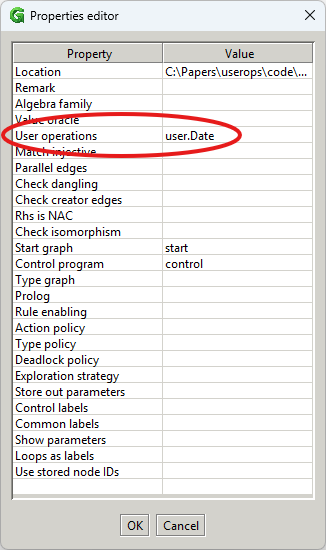
\includegraphics[scale=.55,trim={0 10cm 0 0},clip]{figs/system-properties}
\vspace*{-5mm}
\end{wrapfigure}
To use annotation-defined operators, a rule system has to specify the qualified names of the annotated classes in its System Properties. From then on, they can be treated like built-in system operators.

\Cref{fig:rules} shows two example \GROOVE rules using the operators of \Cref{fig:Date}.
%
\begin{figure}
\subcaptionbox{\createR: a \DateL-typed node is transformed to a \PersonL}[.6\textwidth]{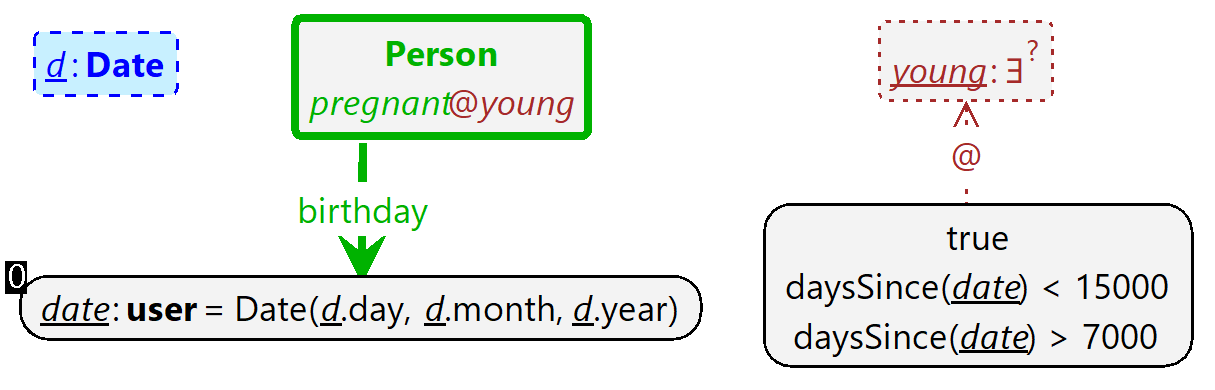
\includegraphics[scale=.17]{figs/create}}
\subcaptionbox{\birthR: a \pregnantL \PersonL gives birth}[.4\textwidth]{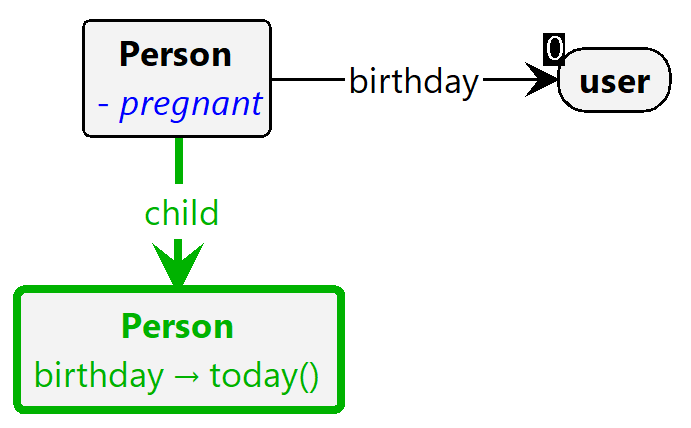
\includegraphics[scale=.17]{figs/birth}}
\caption{\GROOVE rules using the operators defined in \Cref{fig:Date}}
\label{fig:rules}
\end{figure}

\begin{itemize}
\item \createR consumes a node $d$ of (node) type \DateL and invokes the user-defined constructor \code{Date}, using $d$'s node attributes as arguments. It then creates a node of type \PersonL with that \code{Date} as their \birthdayL. Moreover, the created \PersonL is \pregnantL depending on a further condition, specified by the conditional quantifier \youngL: this is satisfied if the number of days since the \birthdayL is properly between 7000 and 15000.

\item \birthR specifies that a \pregnantL person gives birth (and stops being \pregnantL). The newly born \PersonL is a \childL of the first, and its \birthdayL is based on the outcome of the \todayO operator.
\end{itemize}
%
In both rules, the decoration \colorbox{black}{\color{white}0} marks data nodes that serve as \emph{rule parameters} (with number 0, meaning the first --- here: only --- parameter). Parameter values are part of in the transition label when the rule gets applied. An example exploration is shown in \Cref{fig:exploration}: from the start graph on the left, using any of the rule application sequences of the transition system in the middle, eventually the final graph on the right is obtained. The indeterminacy of \todayO causes the outcome of the exploration to depend on the day of execution.
%
\begin{figure}[t]%
\subcaptionbox{Start graph}[.2\textwidth]{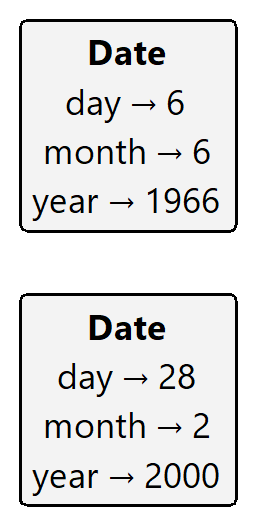
\includegraphics[scale=.17]{figs/start}}%
\subcaptionbox{Transition system}[.55\textwidth]{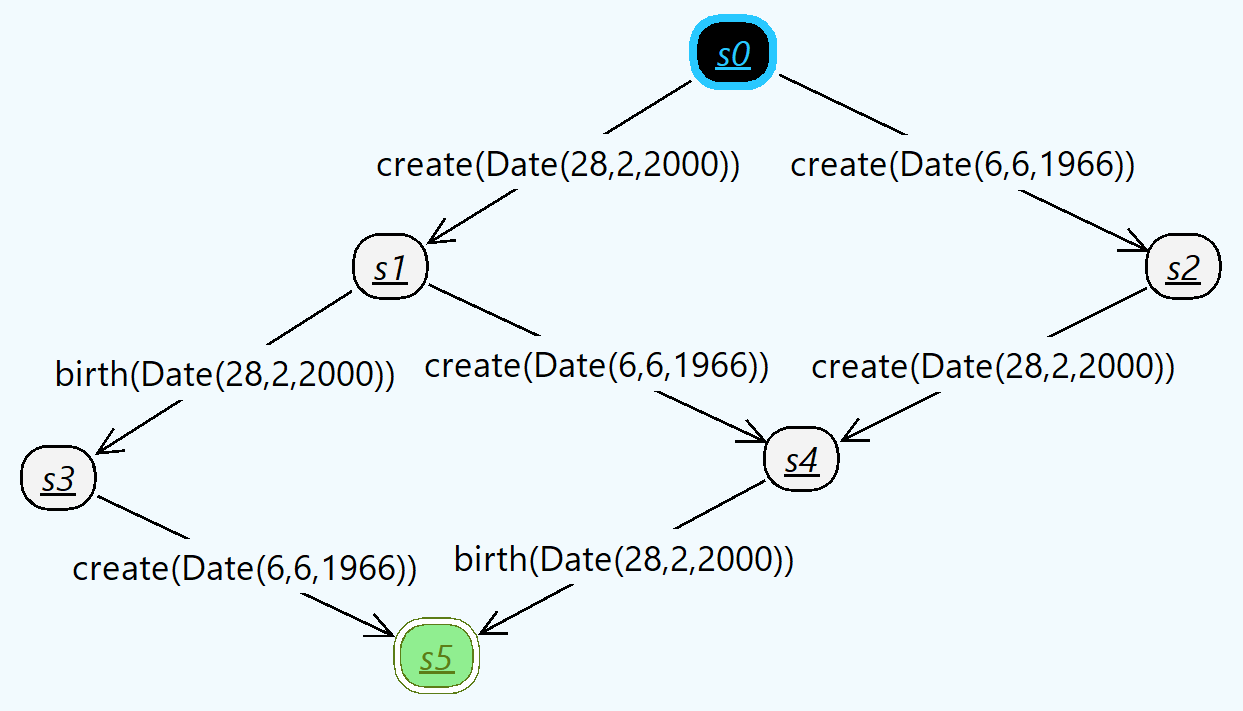
\includegraphics[scale=.14]{figs/user-gts}}%
\subcaptionbox{Final graph}[.25\textwidth]{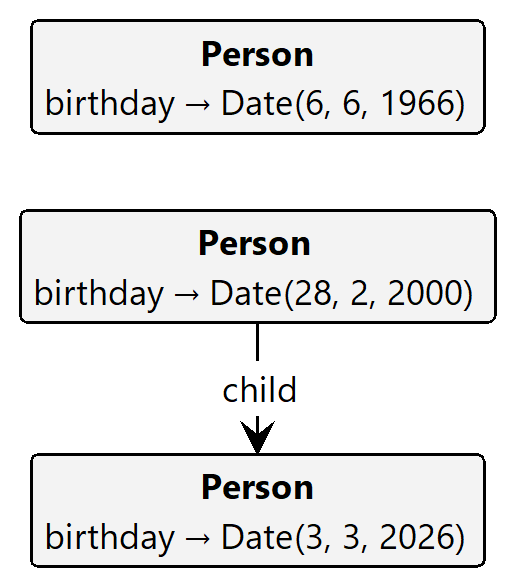
\includegraphics[scale=.17]{figs/final}}
\caption{Example exploration based on the rules in \Cref{fig:rules}}
\label{fig:exploration}
\end{figure}



